\vspace*{1mm}
In 2018, two prototype Crab Cavities ($\CC$s) were installed in the SPS to be tested for the first time with proton beams. One of the operational issues that needed to be addressed concerned the expected emittance growth due to noise in their RF control system. A theoretical model that describes this emittance growth had already been developed and validated by tracking simulations~\cite{PhysRevSTAB.18.101001}. Based on those studies a dedicated experiment was performed to benchmark the models with experimental data and to confirm the analytical predictions. In particular, the idea was to inject various noise levels in the $\CC$ RF system and record the emittance evolution. In this chapter, the experimental procedure, the measurement methods and results are presented and discussed.
 
The chapter is stractured as follows: Section~\ref{sec:CC_SPS_setup} describes the operational setup for the SPS $\CC$ tests and discusses the main diagnostic deployed for the derivation of the $\CC$ voltage.

blah blah ... describe sections and subsections after they are completed.

blah blah ... describe sections and subsections after they are completed.

blah blah ... describe sections and subsections after they are completed.

\section{Crab Cavities in the SPS}\label{sec:CC_SPS_setup}

For the SPS tests two prototype $\CC$s of the Double Quorter Wave (DQW) type were fabricated by CERN and were assembled into the same cryomodule~\cite{Zanoni:2017}. The cryomodule was installed in the SPS-LSS6 zone and was placed on a mobile transfer table~\cite{Garlaschè:2648553}. The table moved with high precision and without breaking the vaccum the cryomodule in the beam line for the $\CC$ tests and out of it for the usual SPS operation. For the emittance growth measurements only one of these $\CC$s was used and its main optics and desgin parameters are listed in Table~\ref{tab:SPS_CCs}. 

\begin{table}[!hbt]
   \centering
   \caption{CC parameters during the SPS emittance growth tests}
   \begin{tabular}{lc}
       \toprule
       \textbf{Parameters} & \textbf{Values}\\
       \bottomrule
       crabbing plane & vertical \\
       $\s$-location & 6313.32\,m \\
      $\fCC$  & 400\,MHz   \\ 
      $\phiCC$  & 0\,deg   \\ 
      \bottomrule
      $\beta_{x, \CC}$, $\beta_{y, \CC}$  & 30.31\,m,  73.82\,m \\
      $\alpha_{x, \CC}$, $\alpha_{y, \CC}$  & tbf \,m,  tbf \,m \\
      $D{x, \CC}$, $D_{y, \CC}$  & tbf \,m,  0 \,m \\     
      \bottomrule
   \end{tabular}
   \label{tab:SPS_CCs}
\end{table}

\large{\textbf{Operational considerations}}

\normalsize{\textbf{Energy ramp}}\\
SPS recieves the beam at 26\,GeV. It was observed that if the ramp to higher energies was performed with the $\CC$ on, the beam was lost while crossing one of the vertical betatron sidebands due to resonant excitation. Therefore, it was established the energy ramp has to be performed with the $\CC$ off and its voltage must be set up only after the energy of interest has been achieved. It should be noted here that this will be the operational scenario also for the HL-LHC.

\normalsize{\textbf{Crab Cavity - main RF synchronisation}}\\
Another issue of concern was the fact that the $\CC$ operate at the fixed frequency of 400\,MHz while the SPS main RF system operates at 200\,MHz.
In order to make sure that the beam will experience the same effect from the $\CC$ each turn the SPS main RF has to be re-phased such as it becomes synchronous with the crabbing signal. For studies at the injection energy of 26\,GeV this synchronisation took place shortly after the injection. For the emittance growth measurements which were performed at 270\,GeV the synchronisation took place at the end of the ramp shortly after the cavity was switched on.

\subsection{Crab Cavity voltage callibration}
The Head-Tail (HT) monitor was the main diagnostic device used for the measurement of the $\CC$ voltage in the experiment. In the first part of this section some basic information on the instrument and its usage will be discussed. Subsequently the method used for the voltage callibration from its reading will be explained. This method was developed at CERN and is described here for completness of the thesis. All experiemental data presented in this subsection belong to the same set of measurements unless it is stated otherwise. They were performed on ... ay 26 GeV for as the crabbing is stronger and the effect more visible for better understadning. In the last part the results from the 270 geV will also be shown. 

\normalsize{\textbf{The Heat-Tail monitor}}\\
\begin{figure}[h]
   \centering         
   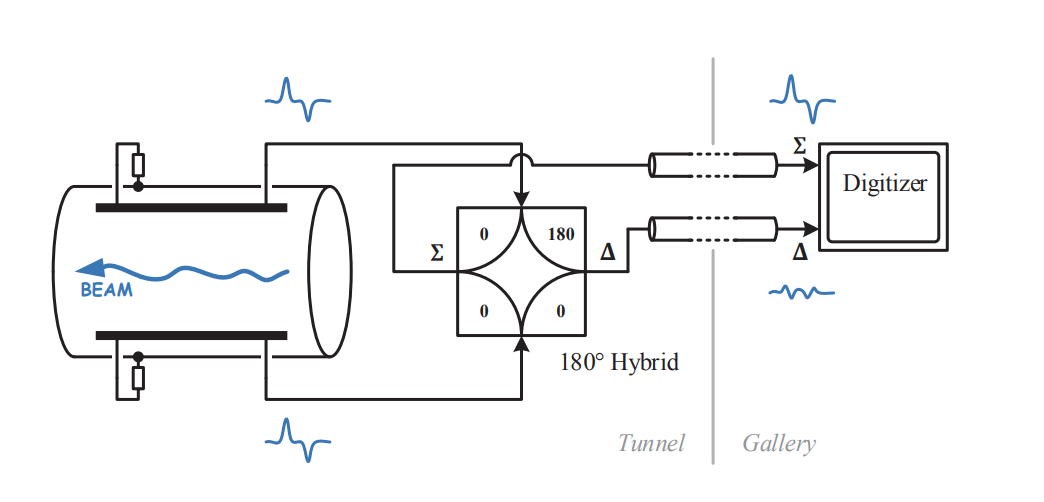
\includegraphics[width=0.8\textwidth]{images/Ch4/SPS_HT_monitor_diagram_modified.png}
       \caption{Diagram of the SPS HT monitor~\cite{Levens:2313358}.}
       \label{fig:SPS_HT_diagram}
\end{figure}
A standard beam position monitor (BPM) measures the bunch centroid position in the transverse planes at every passage of the beam. The HT monitor is a high bandwidth version of a standard BPM and can measure the transverse offset within the bunch, which makes it ideal for the measurement of the crabbing. Its reading consists of the sum $\Sigma$ and the  difference $\Delta$ of the electrode signals of a straight stripline coupler (Fig.~\ref{fig:SPS_HT_diagram})~\cite{Jones:987561, Levens:2313358}. The $\Sigma$ signal is the longitudinal line density while the $\Delta$ signal corresponds to the intra-bunch offset. Example signlas obtained from the HT monitor are displayed in Fig.~\ref{fig:HT_example_acq_singleTurn}-~\ref{fig:HT_example_acq_multTurns_2D}.


\begin{figure}[!h]
   \centering         
   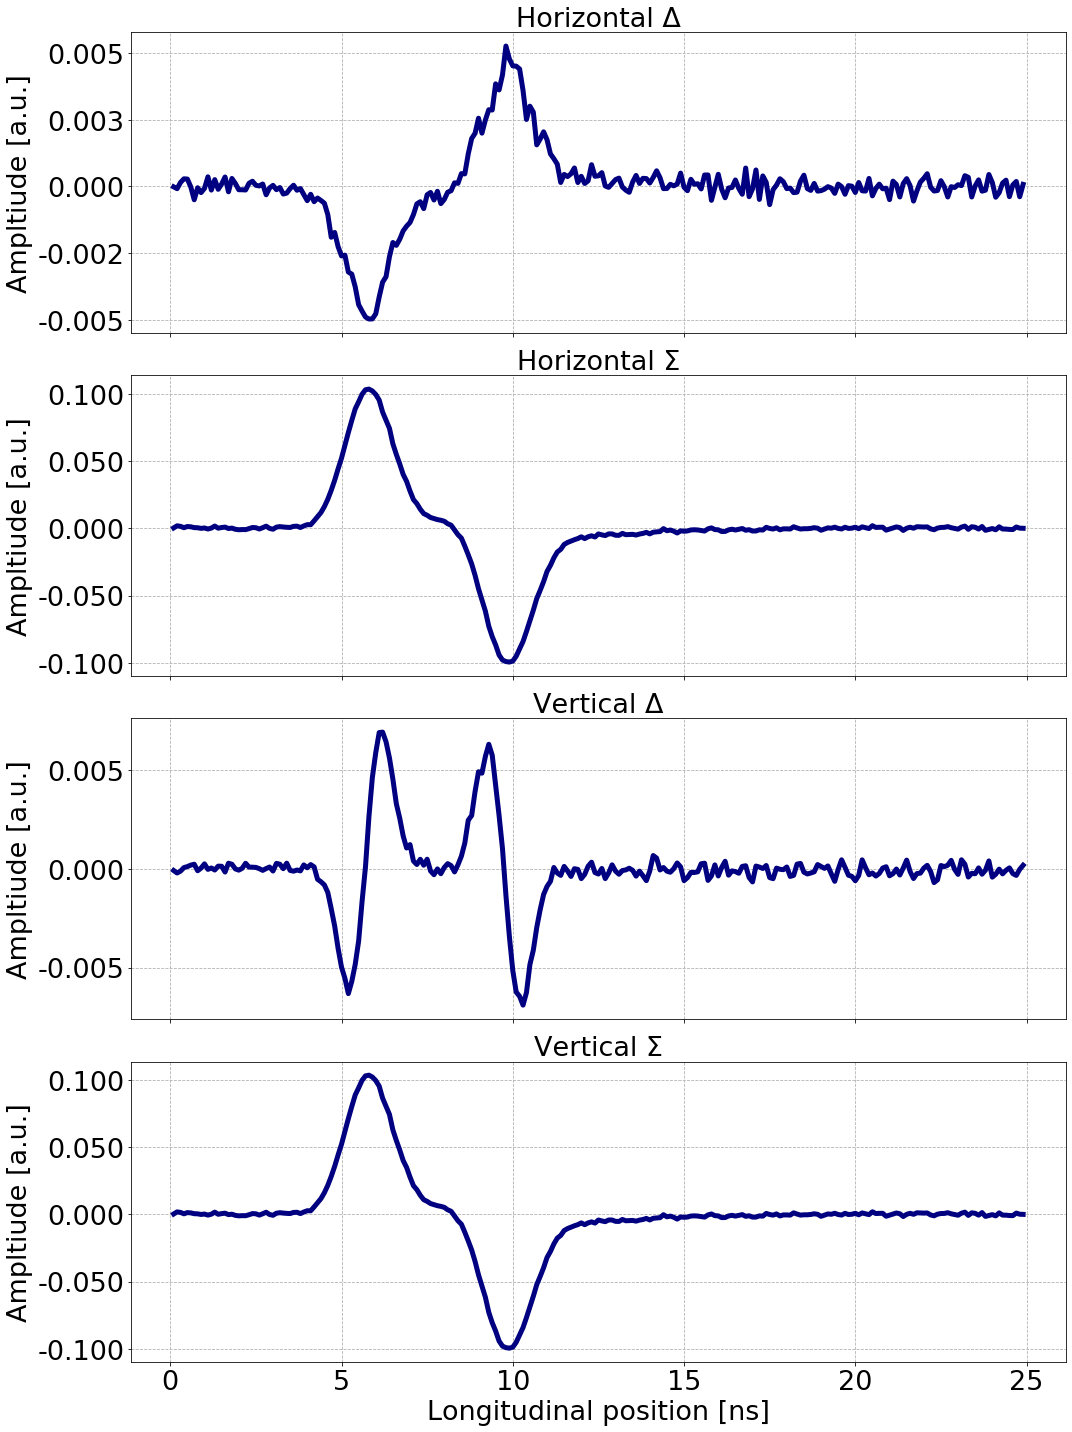
\includegraphics[width=0.8\textwidth]{images/Ch4/HT_1D__20180530_114730_exampleAcq_4thesis_turn3000.png}
       \caption{Raw example $\Delta$ and $\Sigma$ signals obtained from the HT monitor for a window of 25\,ns, acquired in a single SPS revolution.}
       \label{fig:HT_example_acq_singleTurn}
\end{figure}

\begin{figure}[!h]
   \centering         
   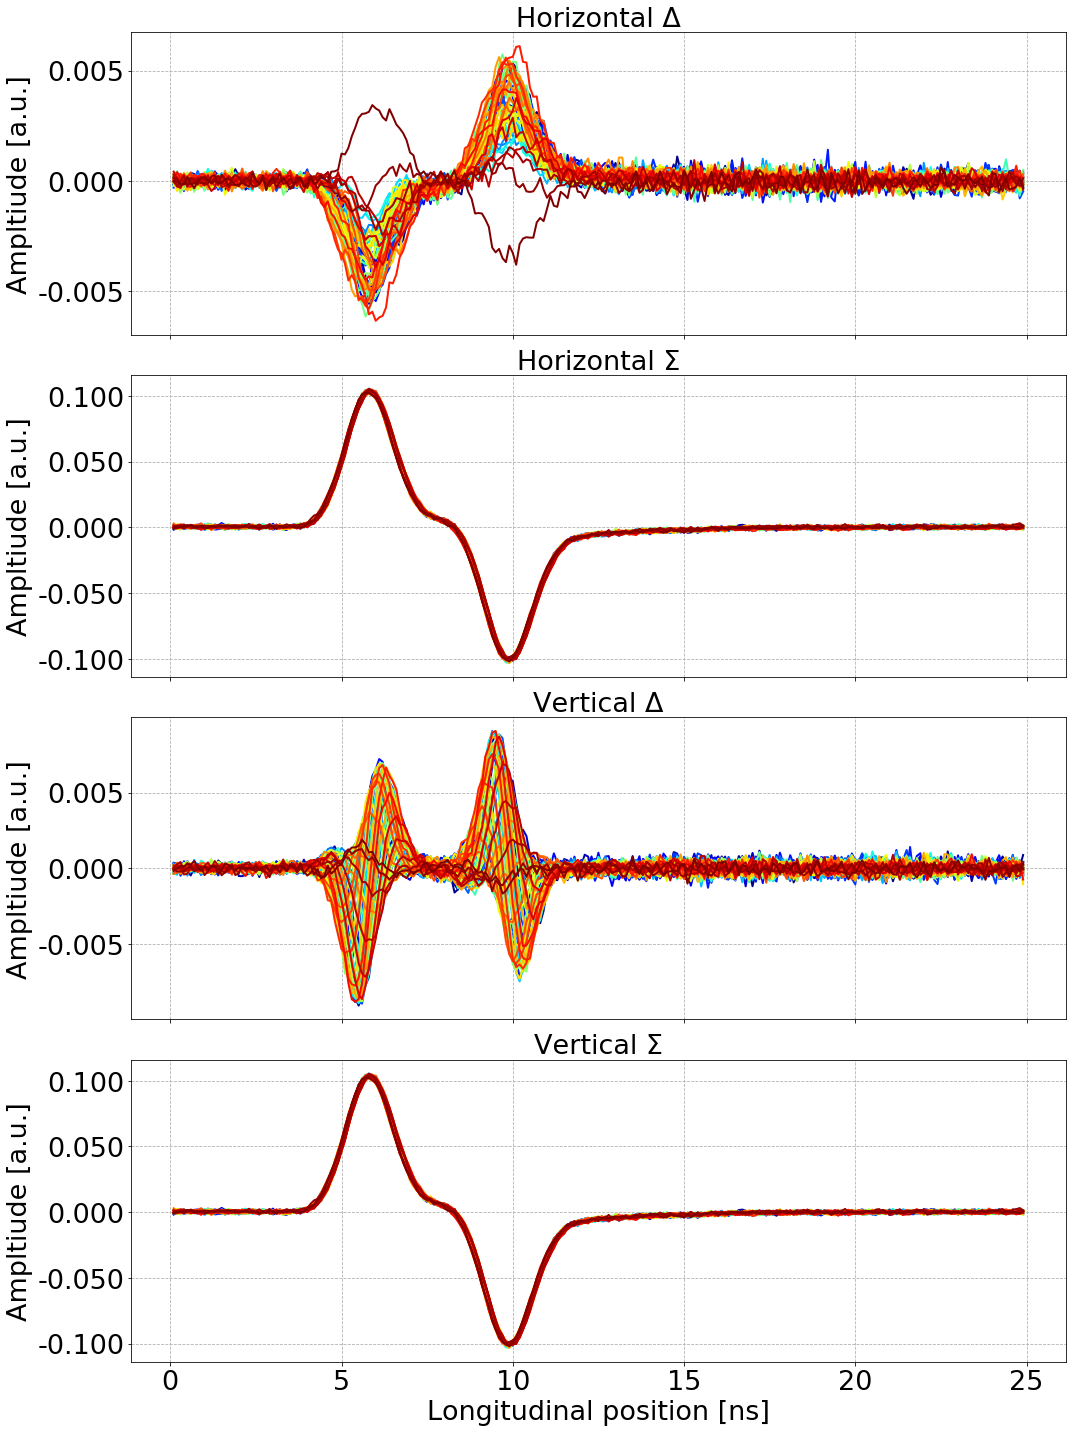
\includegraphics[width=0.8\textwidth]{images/Ch4/HT_1D__20180530_114730exampleAcq_4thesis_turnsStart0_Stop6000_step100.png}
       \caption{Example $\Delta$ and $\Sigma$ signals obtained from the HT monitor for a window of 25\,ns, acquired over several SPS revolutions. The color code indicates the different turns around the machine.}
       \label{fig:HT_example_acq_multTurns}
\end{figure}


\begin{figure}[!h]
   \centering         
   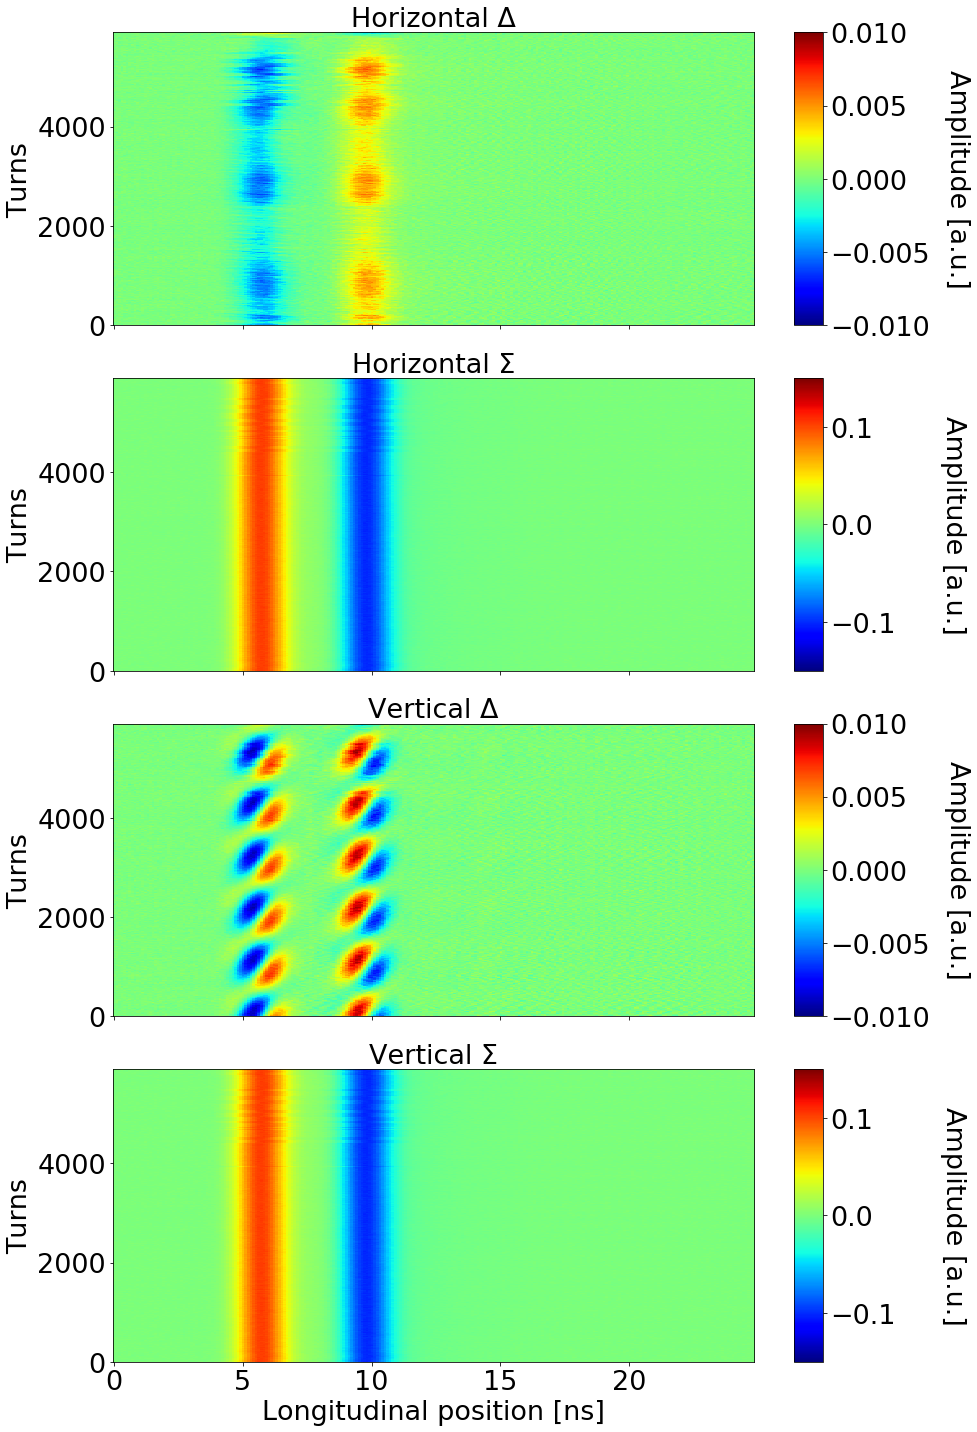
\includegraphics[width=0.8\textwidth]{images/Ch4/HT_2D__20180530_114730_colorbar.png}
       \caption{2D representation of example $\Delta$ and $\Sigma$ signals obtained from the HT monitor for a window of 25\,ns, acquired over several SPS revolutions.}
       \label{fig:HT_example_acq_multTurns_2D}
\end{figure}

In particular, Fig.~\ref{fig:HT_example_acq_singleTurn} and Fig.~\ref{fig:HT_example_acq_multTurns} illustrate the signal acquired over a single and multiple turns of the bunch around SPS respectively. The part of the signal after $\sim$ 9\,ns is just the reflected pulse of the bunch signal from the opposite end of the stripline. Moreover, Fig.~\ref{fig:HT_example_acq_multTurns_2D} shows a 2D representation of the HT monitor reading. In the specific example a clear periodic oscillation of the vertical intra-bunch offset (vertical $\Delta$) signal is observed. This is a result of the main RF system not being synchronous with the  $\CC$  frequency. 


\normalsize{\textbf{Heat-Tail monitor baseline removal}}\\
One issue of concern at that point was the correction of the $\Delta$ signal  baseline due to orbit offsets and non-linearities of the instrument~\cite{Levens:2313358}.  %present due to both the beam orbit offset in the head-tail pick-up and non-linearities of the hybrids, needs to be removed. https://accelconf.web.cern.ch/ibic2016/papers/thal02.pdf
Normally, the baseline is removed by computing the mean of the $\Delta$ signals over all turns and then subtracting this mean from the signal of each turn. However, as already discussed, for the emittance growth measurements the $\CC$ was well synchronised with the main RF system. This resulted in a static intra-bunch position offset which is the signal of interest. By removing the baseline with the method described above the signal of intereset would also be removed.


Therefore, in the SPS experiments a reference measurement had first to be made with the $\CC$ unsynchronised. The mean of the $\Delta$ signal over this reference period was the baseline which then was subtracted from the $\Delta$ signals acquired after the synchronisation (Fig~\ref{fig:HT_baseline_correction}). The datasets before and after synchronisation are easily detectable in the 2D HT monitor reading as displayed in Fig.~\ref{fig:HT_baseline_correction_measurements_2D}

\begin{figure}[!h]
   \centering         
   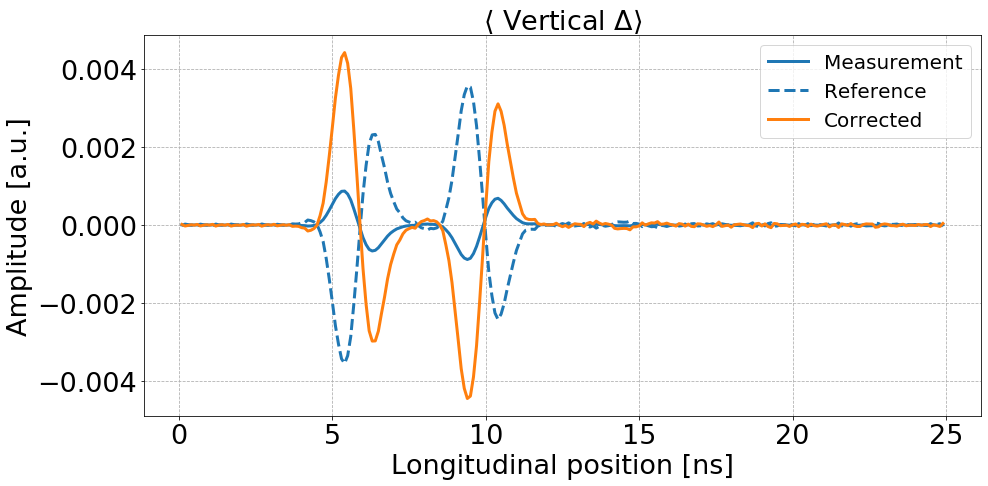
\includegraphics[width=0.8\textwidth]{images/Ch4/HT_measures_vs_reference_vs_corrected__20180530_114730_baseline_correction.png}
       \caption{HT monitor baseline correction for the SPS CC tests.}
       \label{fig:HT_baseline_correction}
\end{figure}

\begin{figure}[!h]
   \centering         
   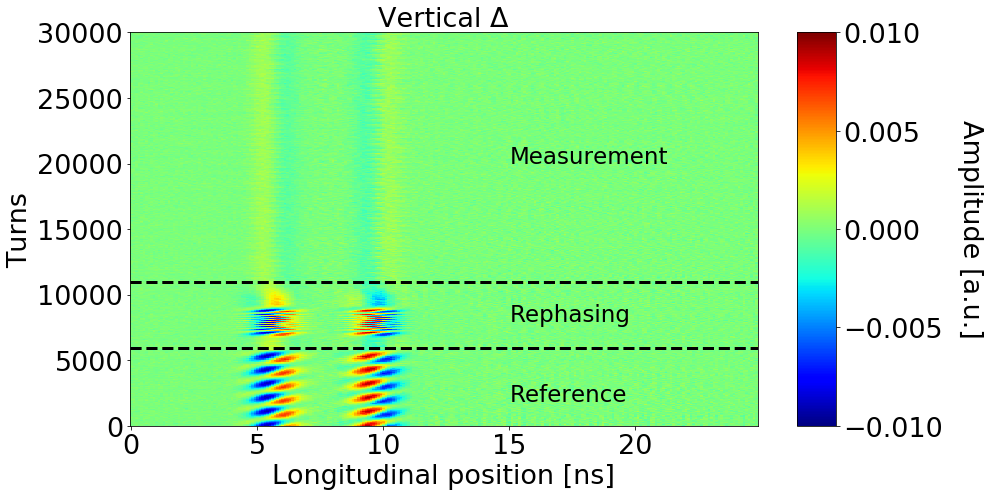
\includegraphics[width=0.8\textwidth]{images/Ch4/HT_measures_vs_reference_vs_corrected__20180530_114730_baseline_correction_onlyDelta.png}
       \caption{HT acquistions before and after the sunchronisation of the SPS main RF with the CC.}
       \label{fig:HT_baseline_correction_measurements_2D}
\end{figure}

\normalsize{\textbf{Headtail monitor callibration}}\\
In order to have the mean intra-bunch offset ($\Delta$) signal in units of \,mm the $\Delta$ acquisitions need to be divided by the $\Sigma$ signal and by a normalisation factor which is computed by the callibration of the HT monitor~\cite{PhysRevAccelBeams.22.112803}. The normalisation factor for the SPS was measured at 0.1052 in 2017. %(T. Levens, private communication)
Figure ... shows the intra bunch offset from the CC kick in mm and after the baseline correction. The reflected part of the signal is discarted here.
 




\normalsize{\textbf{Voltage callibration}}\\
The $\CC$ voltage callibration was performed by calcualting the kick required to reconstruct the intra-bunch offset measurements from the HT monitor. The formula for computing the vertical orbit shift (in meters) from the $\CC$ kick at the HT monitor location $i$ from the $\CC$ kick $\theta$ at the location $j$ is given by~\cite{Carver:2696108, Chao:1490001}:

\begin{equation}
   \Delta y_i  = \frac{\sqrt{\beta_{yi}}}{2 \sin(\pi \Qy)} \theta_j \sqrt{\beta_{yj}} \cos(\pi \Qy - \mid \psi_{yi} - \psi_{yj} \mid),
\end{equation}

where $\beta$ is the beta function, $Q$ is the tune, and $\psi$ is the phase advance in tune units. The same applies for the horizontal plane. The deflection from the $\CC$ can be written as $\theta_j = - \frac{q V(t)}{\symE}$, where q is the charge of the particle, $\symE$ the beam energy and $V(t) = \VCC \sin(2 \pi \fCC t) $ is the voltage that a particle experiences while passing the $\CC$. 

By removing the baseline, callibrating the HT output in mm, and using the corresponding optics 

\normalsize{\textbf{Reconstruction of crabbing}}\\
For completntess


Therefore, the beta function at the 


- The optic information for the ht monitor and the CC are needed.  (mipos na balo edo ta beta functions tou CC)

ty. Therefore in order
to recalculate the kick at the CCs from an offset measurement at an observation point, one only needs information of
the beta-functions and the vertical betatron phases at both
the CCs and the location of the diagnostic device.


\newpage



What is needed --> unsynchronised


\section{Experimental procedure}

\subsection{Machine and beam configuration}
\subsection{Measurement methods}
 What do we measure and how? emittance (show plot ws)
 bunch length ABWLM --> we take the measurement directly from the resposnible tema
 --> show also from the instrument that we saw the unstable bunches.

 \section{Experimental resutls}
 \subsection{Overview}
 - bunches 2, 3 and 4 unstable
 \subsection{Comparison with the theory}

 \newpage 
 This chapter is adapted from the the studies published in Ref.~\cite{Triantafyllou}

 \section{Experimental Setup} % from IPAC paper

Several experimental studies have been performed (2010-2017) to identify the optimal conditions for the emittance growth studies with CCs in the SPS~\cite{Calaga:1451286, Antoniou:2649815}. Based on these preparatory studies, the measurements in the SPS were performed with four low intensity ($\sim 3 \cdot 10^{10}$\, ppb) bunches at 270\,GeV. To minimise the emittance growth from other sources~\cite{Antoniou:2649815} the first order chromaticity, $Q^\prime$, of the machine was corrected to small positive values ($\sim$\,1-2) in both the horizontal and the vertical planes. During the measurements the Landau octupoles were switched off. It should be note, though, that a residual non-linearity was present in the machine mainly due to multipole components in the dipole magnets~\cite{Carlà:2664976, Alekou:2640326}. Only one CC was used, providing a vertical kick to the beam. The transverse feedback system was switched off. Even though the emittance growth is a single bunch effect four bunches were used to reduce the statistical uncertainty of the measurements. The distance between the bunhces was 524 ns. An overview of the relevant SPS parameters during the experiment is given in Table%~\ref{tab:SPS_MD_params}. 


%\begin{table}[!hbt]
%    \centering
%    \caption{SPS parameters during the 2018 MD studies.}
%    \begin{tabular}{lc}
%        \toprule
%        \textbf{Parameters} & \textbf{Values}\\
%       \midrule
%           $E_b$  & 270\,GeV   \\ %[3pt]
%           $\frev$  & 43.375\,kHz  \\ %[3pt]
%           $\nu_x, \nu_y$    & 26.13, 26.18  \\ %[3pt]
%            $\nu_s$ & 0.0051   \\
%            $\VRF$, $\fRF$ & 5\,MV, 200\,MHz \\
%            $\beta_{x, \text{CC}}$, $\beta_{y,\text{CC}}$ &  30.31\,m, 73.82\,m \\
%            $\VCC$, $\fCC$ & 1\,MV, 400\,MHz \\
%       \bottomrule
%    \end{tabular}
%    \label{tab:SPS_MD_params}
% \end{table}

 \subsection{Injected RF noise} 

 In order to characterize the CC noise induced emittance growth, controlled noise was injected into their LLRF system and the evolution of the bunch was recorded for about 20-40 minutes. The injected noise was a mixture of amplitude and phase noise up to 10 KHz, overlapping and primarily exciting the fisrt betatron sideband at $\sim 8$ kHz. The phase noise was always dominant. 